\documentclass[11pt]{article}
\usepackage[margin=1in]{geometry}
\usepackage{booktabs}
\usepackage{array}
\usepackage{graphicx}
\usepackage{enumitem}
\usepackage[htt]{hyphenat}
\sloppy
\usepackage[colorlinks=true,urlcolor=blue,linkcolor=black]{hyperref}

\title{Wearables and Habits: Data Audit, Variable Construction and Balance\\\large Issue \#5}
\date{4 October 2026}
\author{}

\begin{document}
\maketitle

\section{Summary}
Exploratory audit of Open e-commerce 1.0. Main takeaways:
\begin{itemize}[nosep]
\item \textbf{Usable window is 2018-01 to 2023-03, not 2024-08.} Users are observed from their first to last purchase, and almost every window ends by early 2023 (a single user remains after 2023-03). Calendar series are restricted to months with $\geq$1{,}000 active users.
\item \textbf{Treatment (updated, kids' trackers excluded):} 940 users buy a non-kids tracker or smartwatch (Amazon categories \texttt{WEARABLE\_COMPUTER}, \texttt{BIOMETRIC\_MONITOR}); 570 have $\geq$12 months of pre and post history. A stricter ``clean'' definition leaves 723 users (447 with $\geq$12m pre and post).
\item \textbf{Series are smooth in levels} after the restriction (no month-to-month jumps beyond $3\,\mathrm{sd}$ except for one running-shoe month), but rare-event counts (wearable, running shoes, fitness gear) are noisy month to month, as expected from small counts.
\item \textbf{Balance fails.} Ever-treated users differ from never-treated users on income, education, household size and, strongly, on how long they are observed and how much they buy. Adopters are also on a rising purchasing trend before adoption. This supports the plan's main threat (selection and anticipation); the design must use never-treated/not-yet-treated comparisons conditional on covariates, and event-study pre-trends are the key test.
\item \textbf{Data-quality flags (details in the next-to-last section):} Category/Title are missing for 10\% of rows in 2018 but 1\% in 2022, so keyword-based outcomes are undercounted early and part of the upward trends in all flagged series is artificial; the running keyword flag is noisy (only about a fifth of flagged rows are shoes); 37\% of users have a gap of more than 180 days between purchases.
\item The running proxy is only a purchase proxy and is weak in count terms (about 1 in 100 user-months has a running-shoe purchase).
\end{itemize}

\section{Audit}
\begin{center}\small\begin{tabular}{lr}
\toprule
 & Value \\
\midrule
rows & 1,850,717 \\
users & 5,027 \\
survey users & 5,027 \\
purchase users not in survey & 0 \\
missing Category (\%) & 4.83 \\
missing Title (\%) & 4.85 \\
missing price (\%) & 0.00 \\
missing qty (\%) & 0.00 \\
price$\leq$0 rows & 0 \\
qty$>$1 rows (\%) & 5.57 \\
exact duplicate rows & 11,624 \\
date min & 2018-01-01 \\
date max & 2024-08-15 \\
\bottomrule
\end{tabular}
\end{center}
Quirks worth carrying forward: 4.8\% of rows have no Category or Title (they cannot be classified and are treated as non-flagged); 11{,}624 rows are exact duplicates (could be genuine repeat orders, kept, not deduplicated); 5.6\% of rows have quantity above one (spend uses price $\times$ quantity). All 5{,}027 purchasers are in the survey.

\section{Variables built}
The user-month panel (\texttt{code/build/interm/panel\_user\_month.pkl}, gitignored) spans each user's first to last purchase month with zeros filled; $273{,}483$ user-months.
\begin{itemize}[nosep]
\item \textbf{Treatment, non-kids}: first month of a purchase in \texttt{WEARABLE\_COMPUTER} or \texttt{BIOMETRIC\_MONITOR}, dropping titles with kid/child/boy/girl/toddler/junior/``Ace'' (157 of 1{,}598 rows). Watch bands and plain \texttt{WATCH} are excluded (the latter mixes in non-smart watches).
\item \textbf{Treatment, clean}: non-kids, unit price $\geq\$40$ (drops pedometers and cheap knockoffs), quantity one, and title not a compatible/replacement accessory (1{,}086 rows). This is the cleanest ``a real device was bought'' definition; its cost is dropping genuine low-price trackers.
\item \textbf{Medication}: category \texttt{MEDICATION} or \texttt{OTC\_MEDICATION} (human drugs, 16{,}278 rows; animal medication excluded). Titles are mostly OTC (pain, cold, allergy), not prescriptions.
\item \textbf{Running-shoe}: category \texttt{SHOES} or \texttt{TECHNICAL\_SPORT\_SHOE} with a running keyword in the title (2{,}490 rows).
\item \textbf{Running-related} (broader): any running/runner/jogging keyword in the title outside table runners, books and movies, plus \texttt{TECHNICAL\_SPORT\_SHOE} (12{,}342 rows). It includes socks, shorts and headphones, so it is loose; keep both versions.
\item \textbf{Fitness gear}, \textbf{supplements} (secondary or placebo-type outcomes), total purchases and spend (activity controls). Each is a count and a $>0$ dummy per user-month.
\end{itemize}
\begin{center}\small\begin{tabular}{lrrr}
\toprule
 & Mean & Sd & Pct zero \\
\midrule
Purchases & 6.767 & 10.747 & 27.035 \\
Spend (\textbackslash \$) & 161.084 & 292.261 & 27.035 \\
Wearable purchases (non-kids) & 0.005 & 0.082 & 99.514 \\
Wearable purchases (clean) & 0.004 & 0.071 & 99.633 \\
Running-related purchases & 0.045 & 0.271 & 96.451 \\
Running-shoe purchases & 0.009 & 0.115 & 99.234 \\
Fitness-gear purchases & 0.025 & 0.189 & 97.893 \\
Supplement purchases & 0.138 & 0.559 & 91.162 \\
Medication purchases & 0.060 & 0.337 & 95.648 \\
\bottomrule
\end{tabular}
\quad\begin{tabular}{lr}
\toprule
 & Users \\
\midrule
All users & 5027 \\
Ever bought wearable (non-kids) & 940 \\
\quad $\geq$6m pre-history & 854 \\
\quad $\geq$12m pre and post & 570 \\
\quad $\geq$24m pre and post & 165 \\
Ever bought clean wearable & 723 \\
\quad $\geq$12m pre and post & 447 \\
\bottomrule
\end{tabular}
\end{center}
The wearable share is tiny per user-month, so any event-study on a single month will be noisy; bins of 3 months or a dummy outcome over a longer window will probably be needed.

\section{Aggregate series and smoothness}
Medication purchases are smooth and trend up (about 25 to 100 per 1{,}000 users over 2018--2022), as does almost everything else in the panel. The clean wearable series is noisier than the non-kids one because it is a smaller count.
\begin{figure}[h]\centering
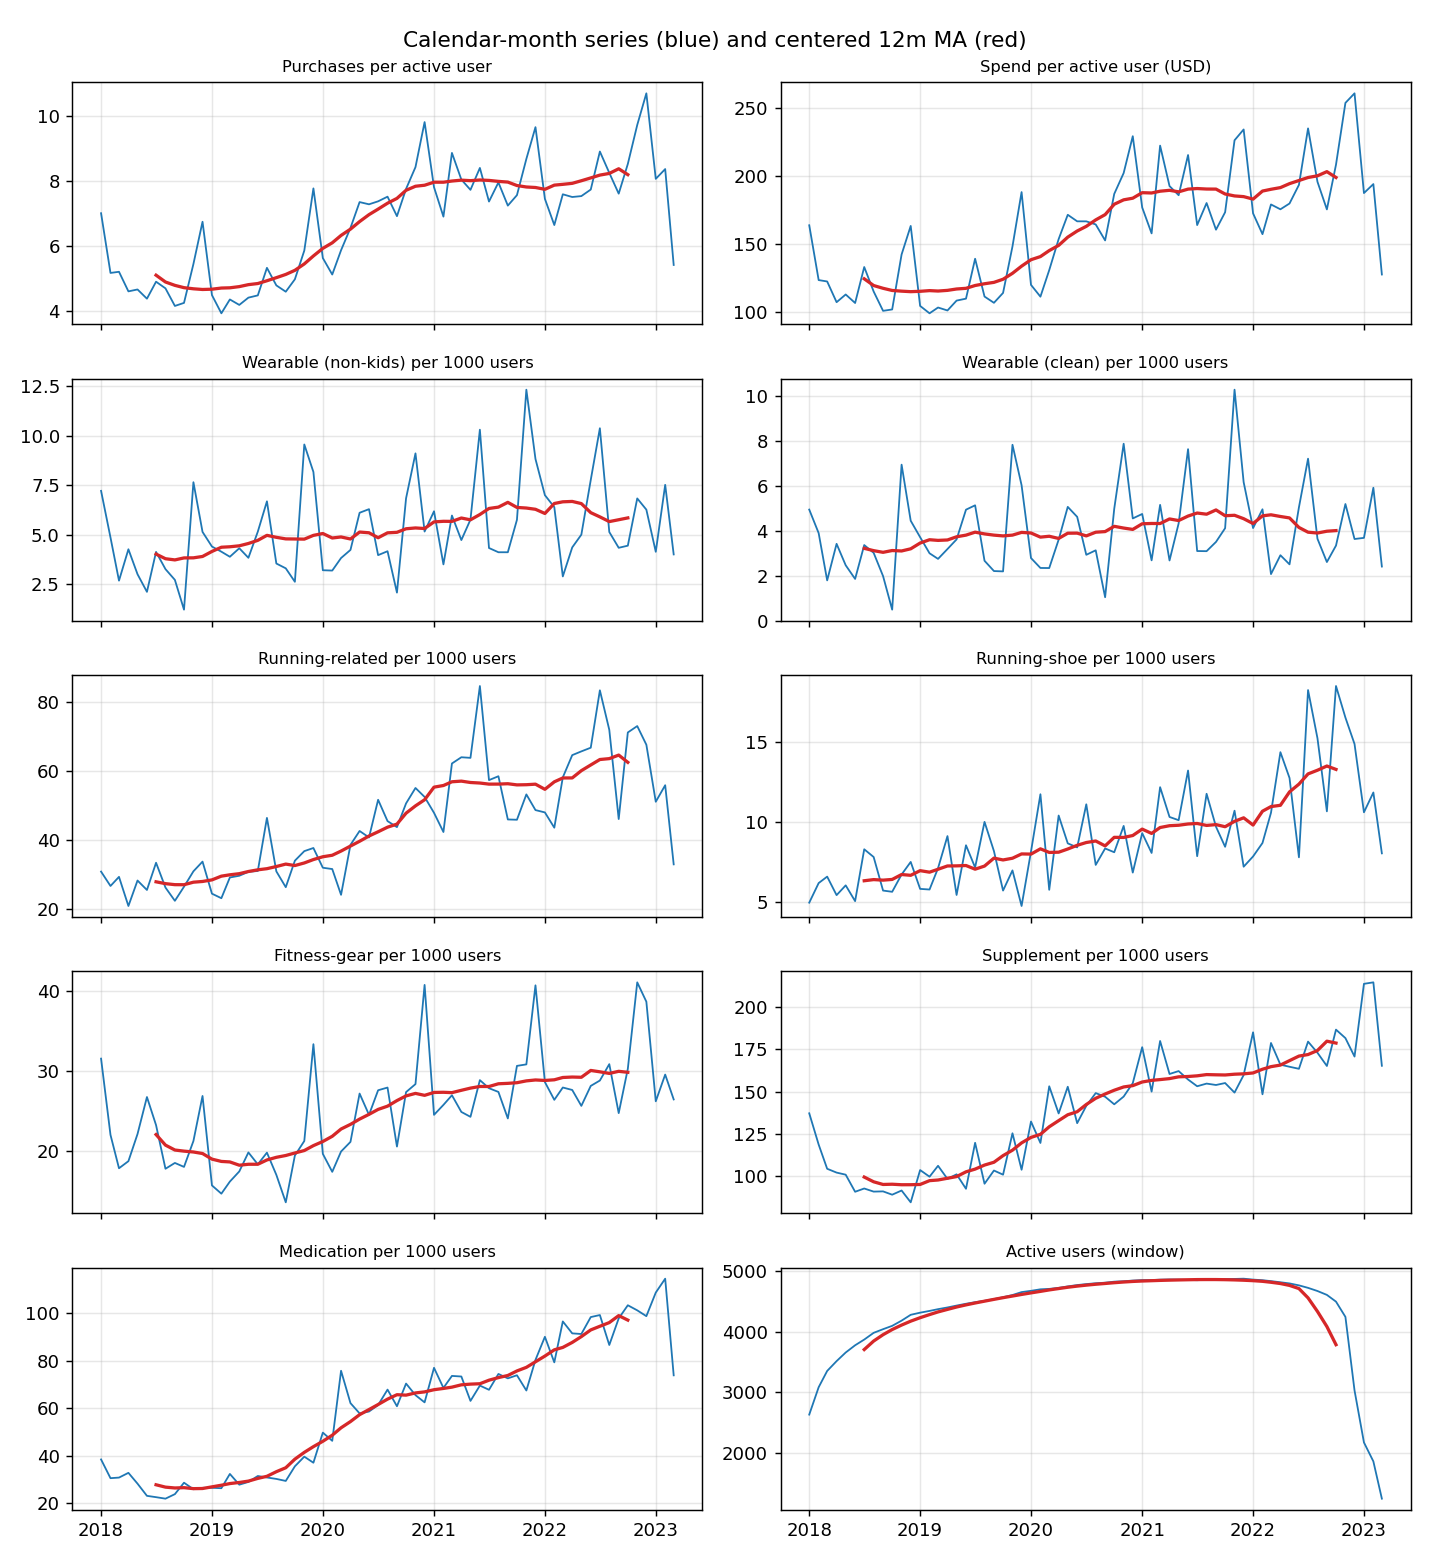
\includegraphics[width=\textwidth]{../code/analysis/outputs/audit_calendar_series.png}
\caption{Calendar-month series per active user (or per 1{,}000 active users) for each constructed variable, with centered 12-month moving average.}
\end{figure}
\begin{center}\small\begin{tabular}{lrrrr}
\toprule
 & Mean & Sd(diff)/Sd(level) & Months $|z|>3$ & AR(1) \\
Series &  &  &  &  \\
\midrule
Purchases per active user & 6.71 & 0.63 & 0 & 0.81 \\
Spend per active user (USD) & 159.83 & 0.72 & 0 & 0.74 \\
Wearable purchases per 1000 users & 5.77 & 1.17 & 0 & 0.32 \\
Running-related per 1000 users & 48.42 & 0.62 & 0 & 0.81 \\
Running-shoe per 1000 users & 9.38 & 0.99 & 1 & 0.51 \\
Fitness-gear per 1000 users & 24.97 & 0.93 & 0 & 0.57 \\
Supplement per 1000 users & 138.42 & 0.51 & 0 & 0.87 \\
Active users & 4,340.89 & 0.29 & 2 & 0.95 \\
\bottomrule
\end{tabular}
\end{center}
All series trend up from 2018 to 2021--22, consistent with growth in purchasing within panel members (and the composition of the panel). Rates are smooth except for the count-based wearable, running-shoe and fitness-gear series, where $\mathrm{sd}(\Delta)/\mathrm{sd}(\mathrm{level})$ is close to one; that is sampling noise, not data breaks. Before restricting to $\geq$1{,}000 active users, the tail had spikes and zeros that come entirely from one or two remaining users; that tail is excluded. The active-user count itself drops sharply after 2022-11, so months after that have a rapidly changing sample.

\begin{figure}[h]\centering
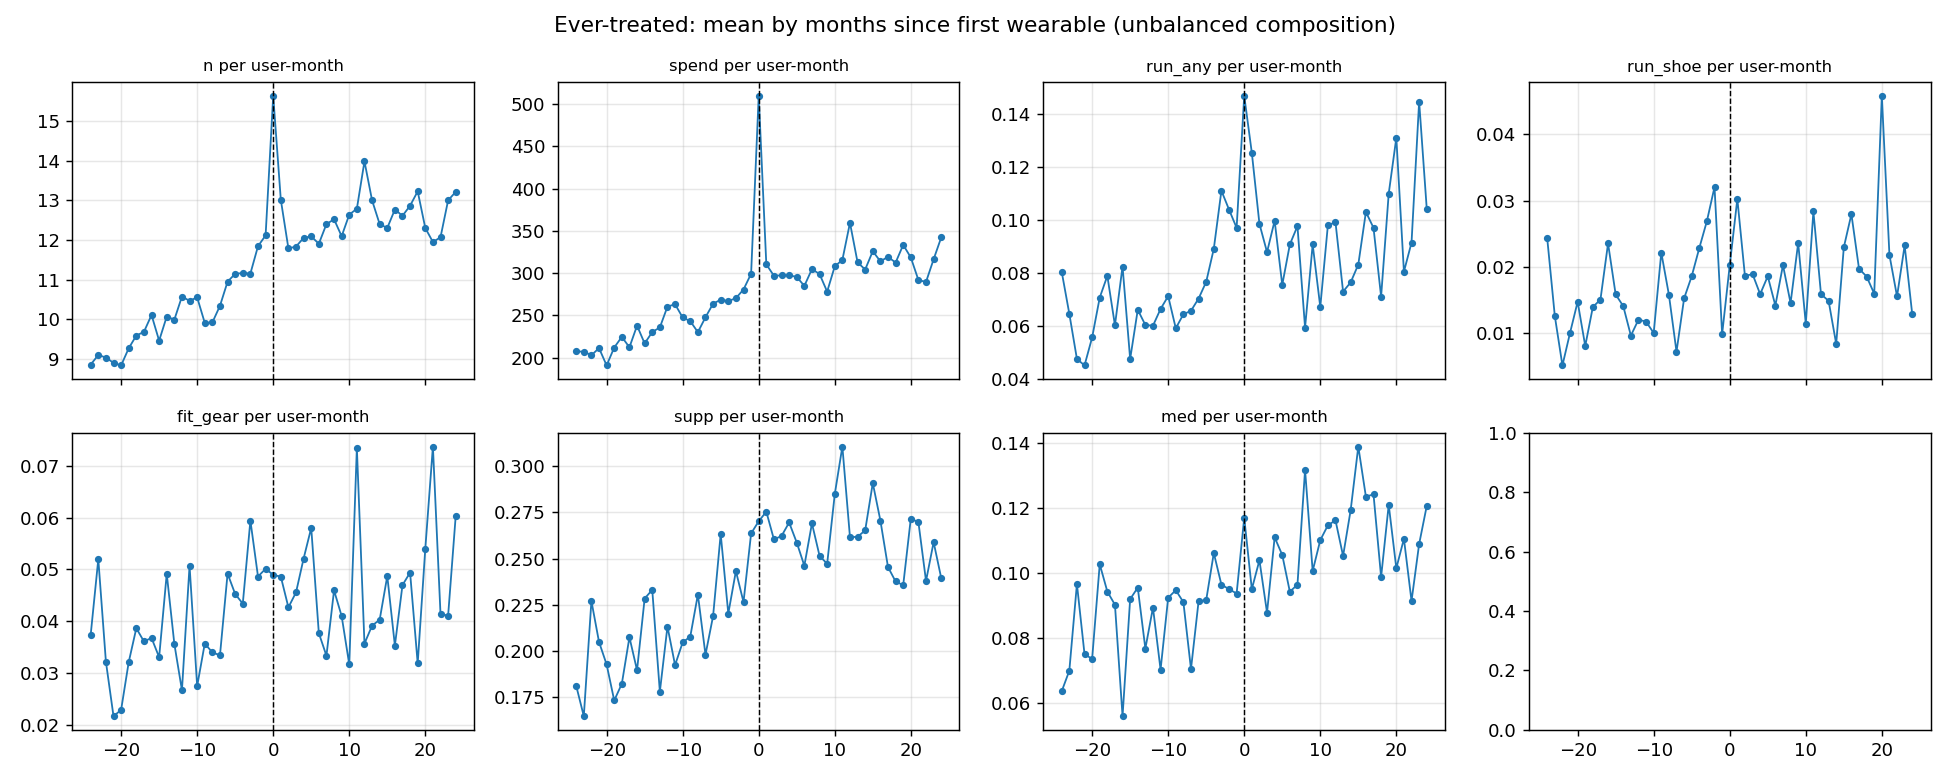
\includegraphics[width=\textwidth]{../code/analysis/outputs/audit_event_time_series.png}
\caption{Ever-treated users: mean outcomes by months since first wearable purchase ($\pm 24$ months; composition changes across event times).}
\end{figure}
Event-time series show (i) a mechanical spike at $t=0$ in total purchases, spend and running-related purchases, because the purchase of the device itself is counted and baskets are bigger around that month, and (ii) a rising pre-adoption trend in purchases, spend, running-related and supplement purchases. The $t=0$ month should be dropped or modeled separately, and the pre-trend must be handled by the control group and the estimator (not-yet-treated comparison). Running-shoe and fitness-gear series are too noisy to read at monthly frequency.

\begin{figure}[h]\centering
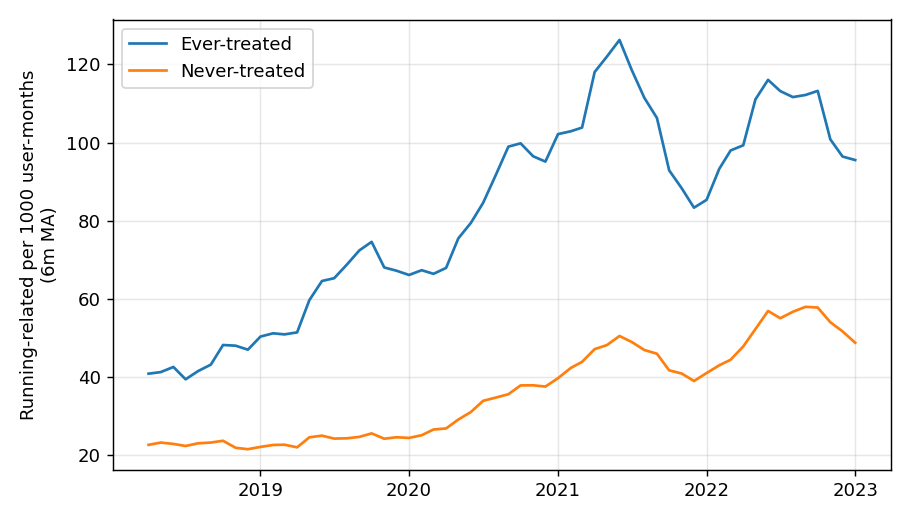
\includegraphics[width=0.6\textwidth]{../code/analysis/outputs/audit_run_treated_vs_never.png}
\caption{Running-related purchases per 1{,}000 user-months, ever-treated versus never-treated (6-month moving average).}
\end{figure}

\section{Correlations}
\begin{figure}[h]\centering
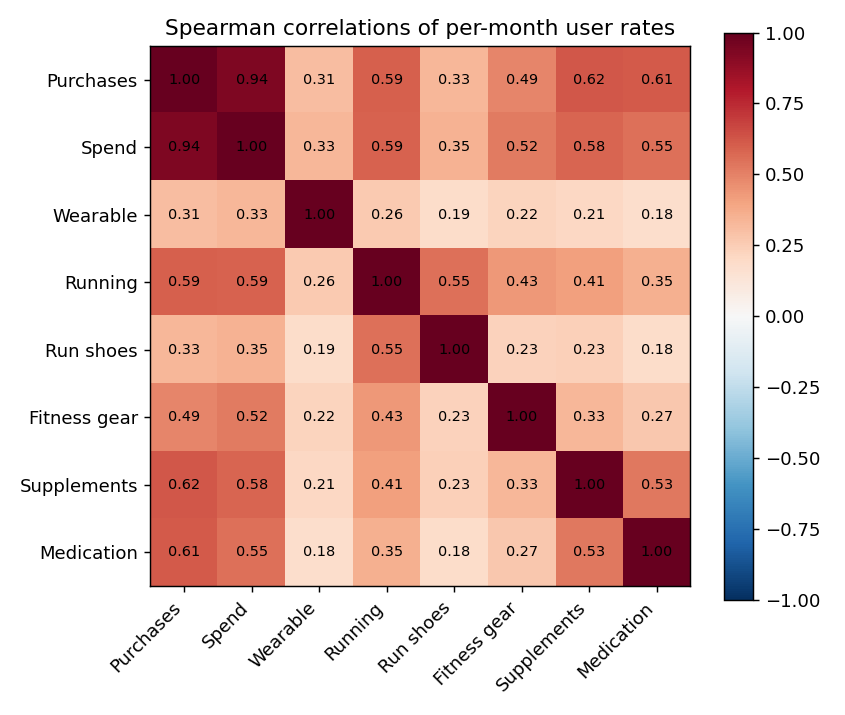
\includegraphics[width=0.6\textwidth]{../code/analysis/outputs/audit_correlations.png}
\caption{Spearman correlations of per-user monthly rates (full observed window).}
\end{figure}
Everything is positively correlated with overall purchasing intensity (running-related 0.59, supplements 0.62, medication 0.61, fitness gear 0.49 with total purchases). The wearable--running correlation (0.26) is no larger than wearable's correlation with supplements (0.21) or fitness gear (0.22), so there is no evident running-specific link at the user level; the raw association is mostly ``heavy buyer'' selection, and outcomes should be conditioned on or scaled by overall activity.

\section{Balance tests}
Linear probability models (HC1 standard errors, covariates standardized so coefficients are the change in $P(\mathrm{ever\ treated})$ per $+1\,\mathrm{sd}$) with joint $F$-tests.
Demographics come from the survey; only the 76 ``prefer not to say'' income answers drop out, so $N=4{,}951$ for the demographic regressions.
\begin{figure}[h]\centering
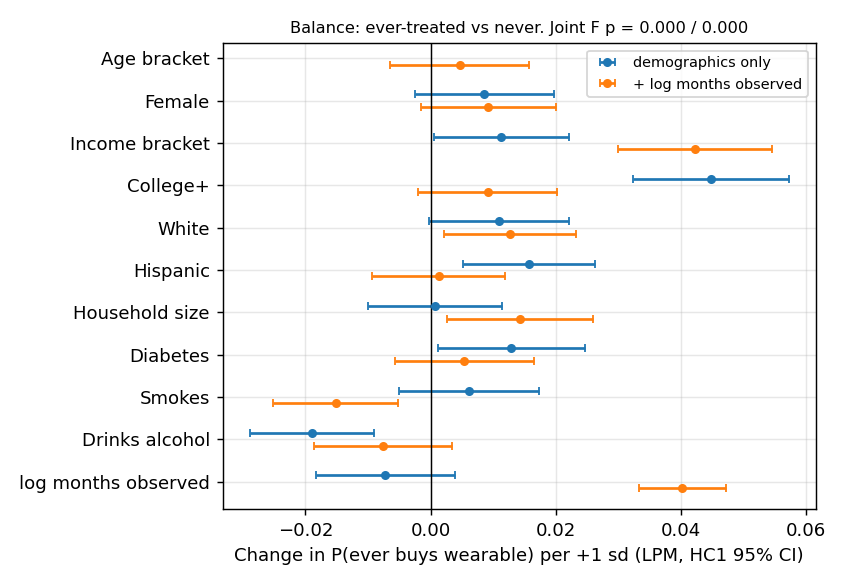
\includegraphics[width=0.75\textwidth]{../code/analysis/outputs/audit_balance_ever_treated.png}
\caption{Ever-treated vs never-treated on survey demographics, with and without log months observed.}
\end{figure}
\begin{figure}[h]\centering
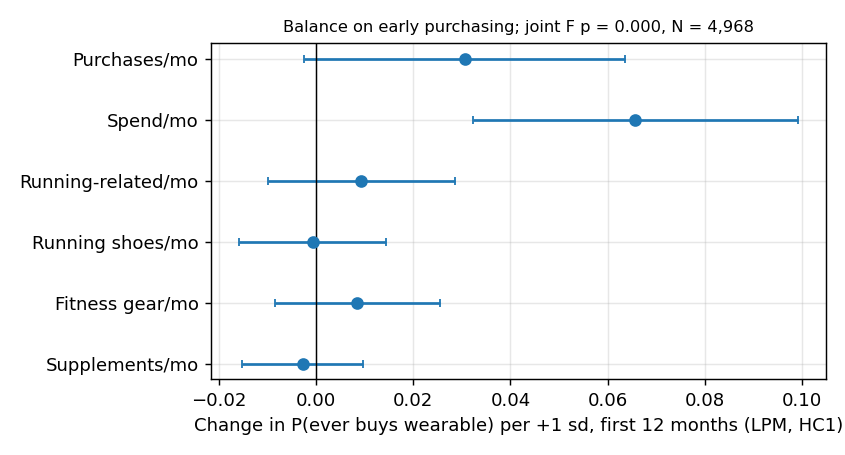
\includegraphics[width=0.75\textwidth]{../code/analysis/outputs/audit_balance_prepurchasing.png}
\caption{Ever-treated on purchasing rates in each user's first 12 observed months.}
\end{figure}
\begin{figure}[h]\centering
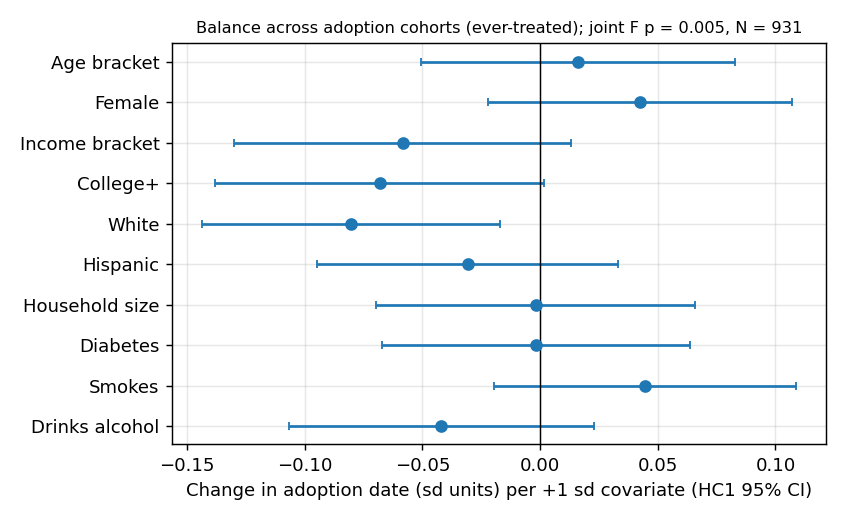
\includegraphics[width=0.75\textwidth]{../code/analysis/outputs/audit_balance_timing.png}
\caption{Among ever-treated users: adoption date on demographics (balance across cohorts).}
\end{figure}
\begin{center}\small\begin{tabular}{lrr}\toprule
Regression & Joint $F$ p-value & N \\\midrule
Ever-treated on demographics & 0.000 & 4,951 \\
Ever-treated on demographics + log months & 0.000 & 4,951 \\
Ever-treated on first-12m purchasing & 0.000 & 4,968 \\
Adoption date on demographics (treated only) & 0.005 & 931 \\
\bottomrule\end{tabular}
\end{center}
All joint tests reject. Treated users have higher income, are more often white and non-smokers, live in larger households, and are observed for longer (age, education and gender are not individually significant) (a $+1\,\mathrm{sd}$ longer window is worth about $+4$ percentage points of adoption probability against a base of about 20\%, which is partly mechanical: more months give more chances to buy). They also buy more overall in their first year. Conditional on overall purchasing and spend, early running, fitness and supplement rates do not predict adoption, but unconditionally ever-treated users buy about twice as many running-related items as never-treated users throughout the sample (the running-related figure above), so the level difference is largely general buying intensity. Cohorts are also not balanced on demographics ($p=0.006$), so timing is not as-good-as-random.

\section{Data quality}
All checks in \texttt{code/scripts/data\_quality\_checks.py}.

\subsection*{Missing classification fields over time}
\begin{center}\small\begin{tabular}{lrrr}
\toprule
 & Rows & Category missing (\%) & Title missing (\%) \\
Year &  &  &  \\
\midrule
2018 & 225,465 & 10.4 & 10.5 \\
2019 & 266,016 & 7.7 & 7.7 \\
2020 & 409,212 & 5.7 & 5.7 \\
2021 & 467,870 & 3.5 & 3.5 \\
2022 & 442,230 & 1.3 & 1.3 \\
2023 & 39,923 & 0.6 & 0.6 \\
2024 & 1 & 0.0 & 0.0 \\
\bottomrule
\end{tabular}
\end{center}
Category and Title are missing together (the same rows), falling steadily from about 10\% of rows in 2018 to about 1\% in 2022. Missing rows are not random: their median price is \$16 versus \$14 for classified rows. Because every outcome and the treatment are defined from Category or Title, all flagged counts are mechanically undercounted early in the sample, which creates an artificial upward trend in every series (visible in the calendar figure). Next issue should either express outcomes as shares of classified purchases or include year effects, and test sensitivity to dropping 2018--2019.

\subsection*{Coverage per user}
\begin{figure}[h]\centering
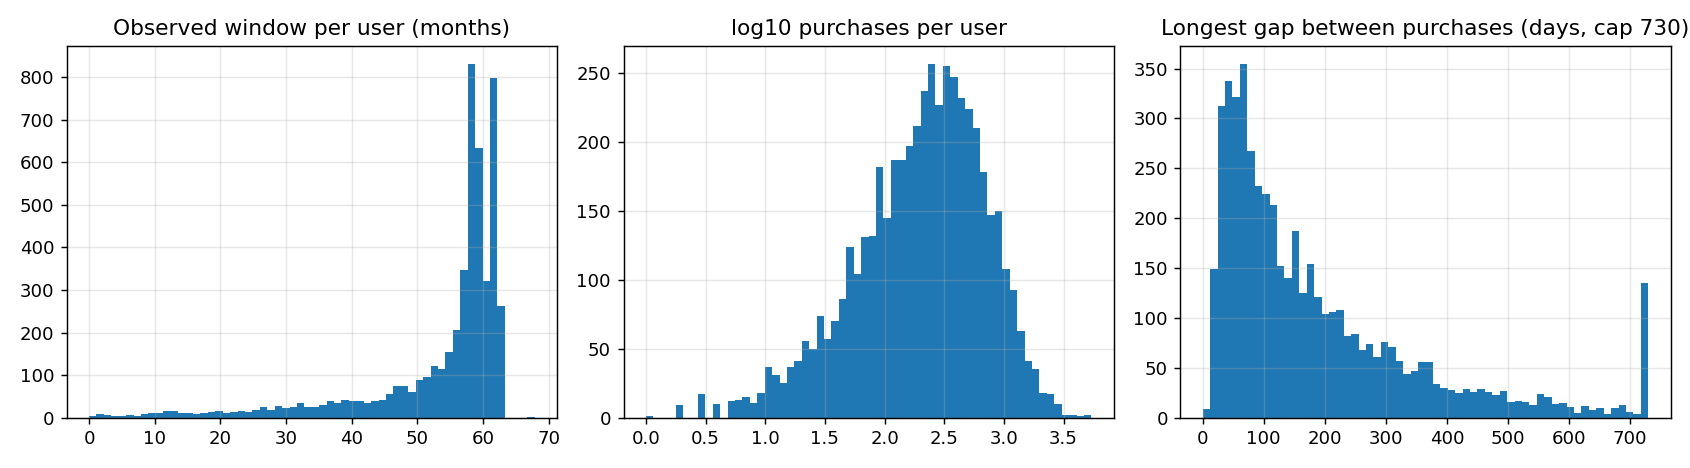
\includegraphics[width=\textwidth]{../code/analysis/outputs/dq_user_coverage.png}
\caption{Observed window, purchases per user and longest gap between purchases.}
\end{figure}
Users are heavy and long-lived (median 232 purchases over 58 months; only 1.6\% are observed under 12 months). But 37\% of users have a gap of more than 180 days, so ``no purchase in a month'' sometimes means ``not shopping on Amazon,'' not ``did not buy''. A zero in the panel is a weak signal for the extensive margin; the next issue could trim long inactive spells.
\begin{figure}[h]\centering
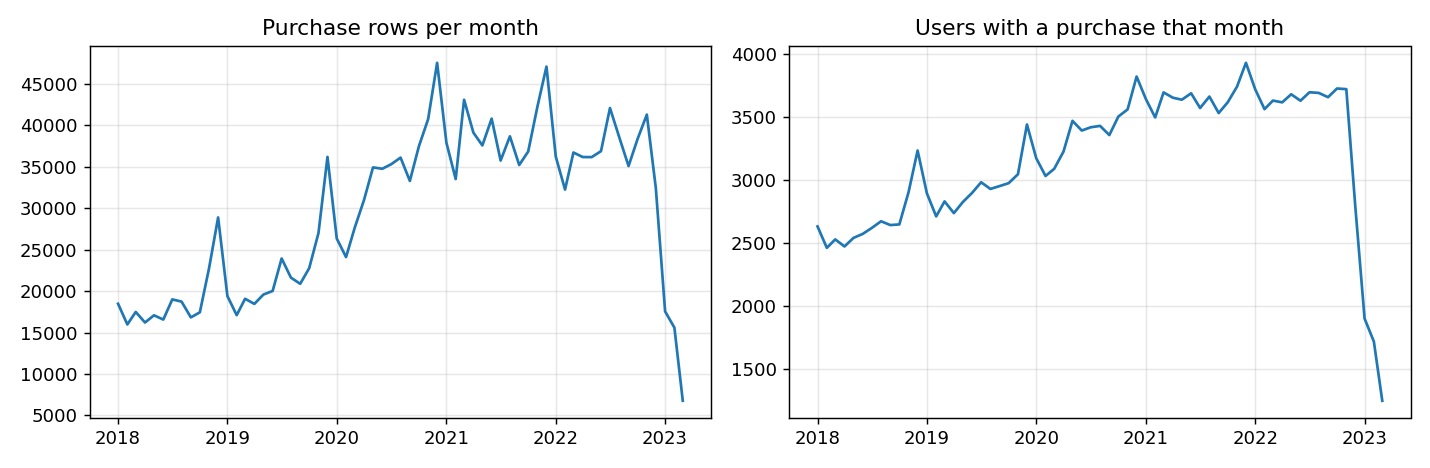
\includegraphics[width=\textwidth]{../code/analysis/outputs/dq_rows_per_month.png}
\caption{Raw purchase rows per month and users with a purchase that month (months with $\geq$1{,}000 users).}
\end{figure}

\subsection*{Duplicates, outliers and other checks}
\begin{center}\small\begin{tabular}{lr}
\toprule
 & Value \\
\midrule
dup rows (all columns) & 21,039 \\
dup share of rows (\%) & 1.1 \\
users with any dup & 3,037 \\
dup rows in top-1\% users (\%) & 30.4 \\
dup share, missing-title rows (\%) & 1.3 \\
dup share, titled rows (\%) & 1.1 \\
dup wearable rows & 5 \\
median window (months) & 58.3 \\
users window <12m (\%) & 1.6 \\
users window <24m (\%) & 4.3 \\
median purchases / user & 232.0 \\
users with <10 purchases (\%) & 2.1 \\
median longest gap (days) & 128.0 \\
users with a gap >180 days (\%) & 37.2 \\
price > \$500 rows & 2,176 \\
price > \$2000 rows & 57 \\
qty >= 10 rows & 1,097 \\
spend > \$5000 rows & 5 \\
share of spend in top 0.1\% rows (\%) & 4.2 \\
wearable rows non-kids / clean & 1,441 / 1,086 \\
non-kids wearables with price < \$40 (\%) & 21.2 \\
run\_any rows in SHOES/TECH SHOE (\%) & 20.6 \\
run\_any rows with 'running shoe' in title (\%) & 17.5 \\
medication rows w/ 'pet|dog|cat' in title (\%) & 0.2 \\
\bottomrule
\end{tabular}
\end{center}
Duplicates (same user, date, price, quantity, title and category) are 1.1\% of rows, spread over 3{,}037 users with 30\% in the top 1\% of users; only 5 are wearable rows, so they are probably repeat or multi-unit orders and are kept. Price and quantity outliers are few and look real (a 96TB drive, 8 batteries); the top 0.1\% of rows hold 4.2\% of spend, so spend should be log-transformed or winsorized.

\subsection*{Validation of the treatment definitions}
\begin{center}\small\begin{tabular}{lrrr}
\toprule
 & Rows & In clean def. & Median price (\$) \\
Brand &  &  &  \\
\midrule
fitbit & 478 & 449 & 113 \\
other / unbranded & 390 & 150 & 40 \\
apple watch & 206 & 194 & 262 \\
samsung & 121 & 101 & 199 \\
garmin & 90 & 78 & 160 \\
amazfit & 48 & 42 & 68 \\
xiaomi & 40 & 15 & 37 \\
fossil & 32 & 32 & 198 \\
polar & 25 & 18 & 72 \\
huawei & 4 & 4 & 61 \\
withings & 4 & 2 & 115 \\
misfit & 2 & 0 & 22 \\
suunto & 1 & 1 & 114 \\
\bottomrule
\end{tabular}
\end{center}
Branded devices are almost all in the clean definition. The unbranded group (390 rows, median price \$40) is where the definitions differ: about a fifth of non-kids wearable rows cost less than \$40 and are mostly generic fitness bands, pedometers and a few non-tracker items (an ankle band, a medical alert device, a heart-rate armband). Some real branded devices fall out of the clean definition (e.g.\ multi-unit orders or titles starting ``for Fitbit''), and the non-kids filter keeps at least one Garmin device that was dropped by the clean rule, so the clean definition is conservative on both sides.

\subsection*{Validation of outcome definitions}
Only 21\% of running-related rows are shoes; the rest are shorts, pants, socks, headphones, waist packs and braces whose title says ``running'', plus some noise (dog running cables, cooling towels). Running-shoe is precise but rare; running-related is a ``sports apparel for running'' measure with false positives. Medication titles are human OTC drugs (pain, allergy, cough, antacid); only 0.2\% mention pets. Prescription drugs are not observed.

\subsection*{Survey}
\begin{center}\small\begin{tabular}{lr}
\toprule
 & Missing / prefer not (\%) \\
\midrule
Q-demos-age & 0.0 \\
Q-demos-race & 0.0 \\
Q-demos-education & 0.6 \\
Q-demos-income & 1.5 \\
Q-demos-gender & 0.2 \\
Q-amazon-use-hh-size & 0.0 \\
Q-substance-use-alcohol & 0.5 \\
Q-personal-diabetes & 0.3 \\
\bottomrule
\end{tabular}
\end{center}
Survey covariates are essentially complete: no missing values in the ten items used, except 76 income answers (1.5\%) coded ``Prefer not to say''. A bug in the first version of the balance regressions silently dropped the 1{,}199 respondents who answered ``1 (just me!)'' to household size (the answer was not numeric), cutting $N$ from 5{,}027 to 3{,}761; it is fixed and the balance results above use the corrected sample. Lesson for the next issue: check the $N$ after every covariate merge.

\section{Go/no-go read and next steps}
\begin{itemize}[nosep]
\item Sample size is workable for a reduced-form design (about 600 treated users with $\geq$12 months pre and post) but thin for monthly running-shoe outcomes. Preliminary read: \textbf{conditional go}, with the broader running measure and quarterly bins as the primary outcome.
\item Needed next: decide how to handle the declining missing-title share (below) and duplicates; decide on the running outcome definition (tighter keyword audit of titles); set up the Callaway--Sant'Anna comparison group (not-yet-treated plus never-treated) with demographics and pre-adoption purchase intensity as covariates; handle the $t=0$ spike and the 2022-11 sample drop.
\item Environment note: the compose \texttt{container\_name: research-container} collides with another project's running container on this machine (mounted from \texttt{exploration-exploitation}), so this audit was run with \texttt{docker compose run} on this repo's \texttt{code-opt} image (same service, no new container). R \texttt{fixest} and \texttt{did} load there; the audit regressions are in Python \texttt{statsmodels} because they are simple LPMs.
\end{itemize}
\end{document}
